\section{The Pair Background Envelopes}
\label{sec:Envelopes}
The beamstrahlung from beam-beam interactions produces secondary \Pep \Pem pairs.
These processes were simulated with \guineapig, a Monte Carlo (MC) background event generator~\cite{Schulte:1997nga}.
For all ILC250 parameter sets, listed in Table~\ref{tab:Parameters}, a full bunch train (1312 bunch crossings) of the pair background particles were generated.
The calculation of the helix tracks that the pairs form in the SiD solenoid field with a strength of \SI{5}{\tesla} was done using the algorithm descibed in a former note presenting the pair envelopes of the ILC500 scheme.~\cite{HelixProceeding}

\iffalse
Figure~\ref{fig:Helixes} shows the helix tracks of the pair background from one bunch crossing in the xz-plane.
With the envelopes drawn in Figures~\ref{fig:envelopes_xz}, it becomes clear that the distance between 99\% of all pair particle tracks and the beam pipe is more than \unit{4}\,{mm} at any given point.


\begin{figure}
    \centering
    \begin{subfigure}[b]{0.49\textwidth}
    \centering
        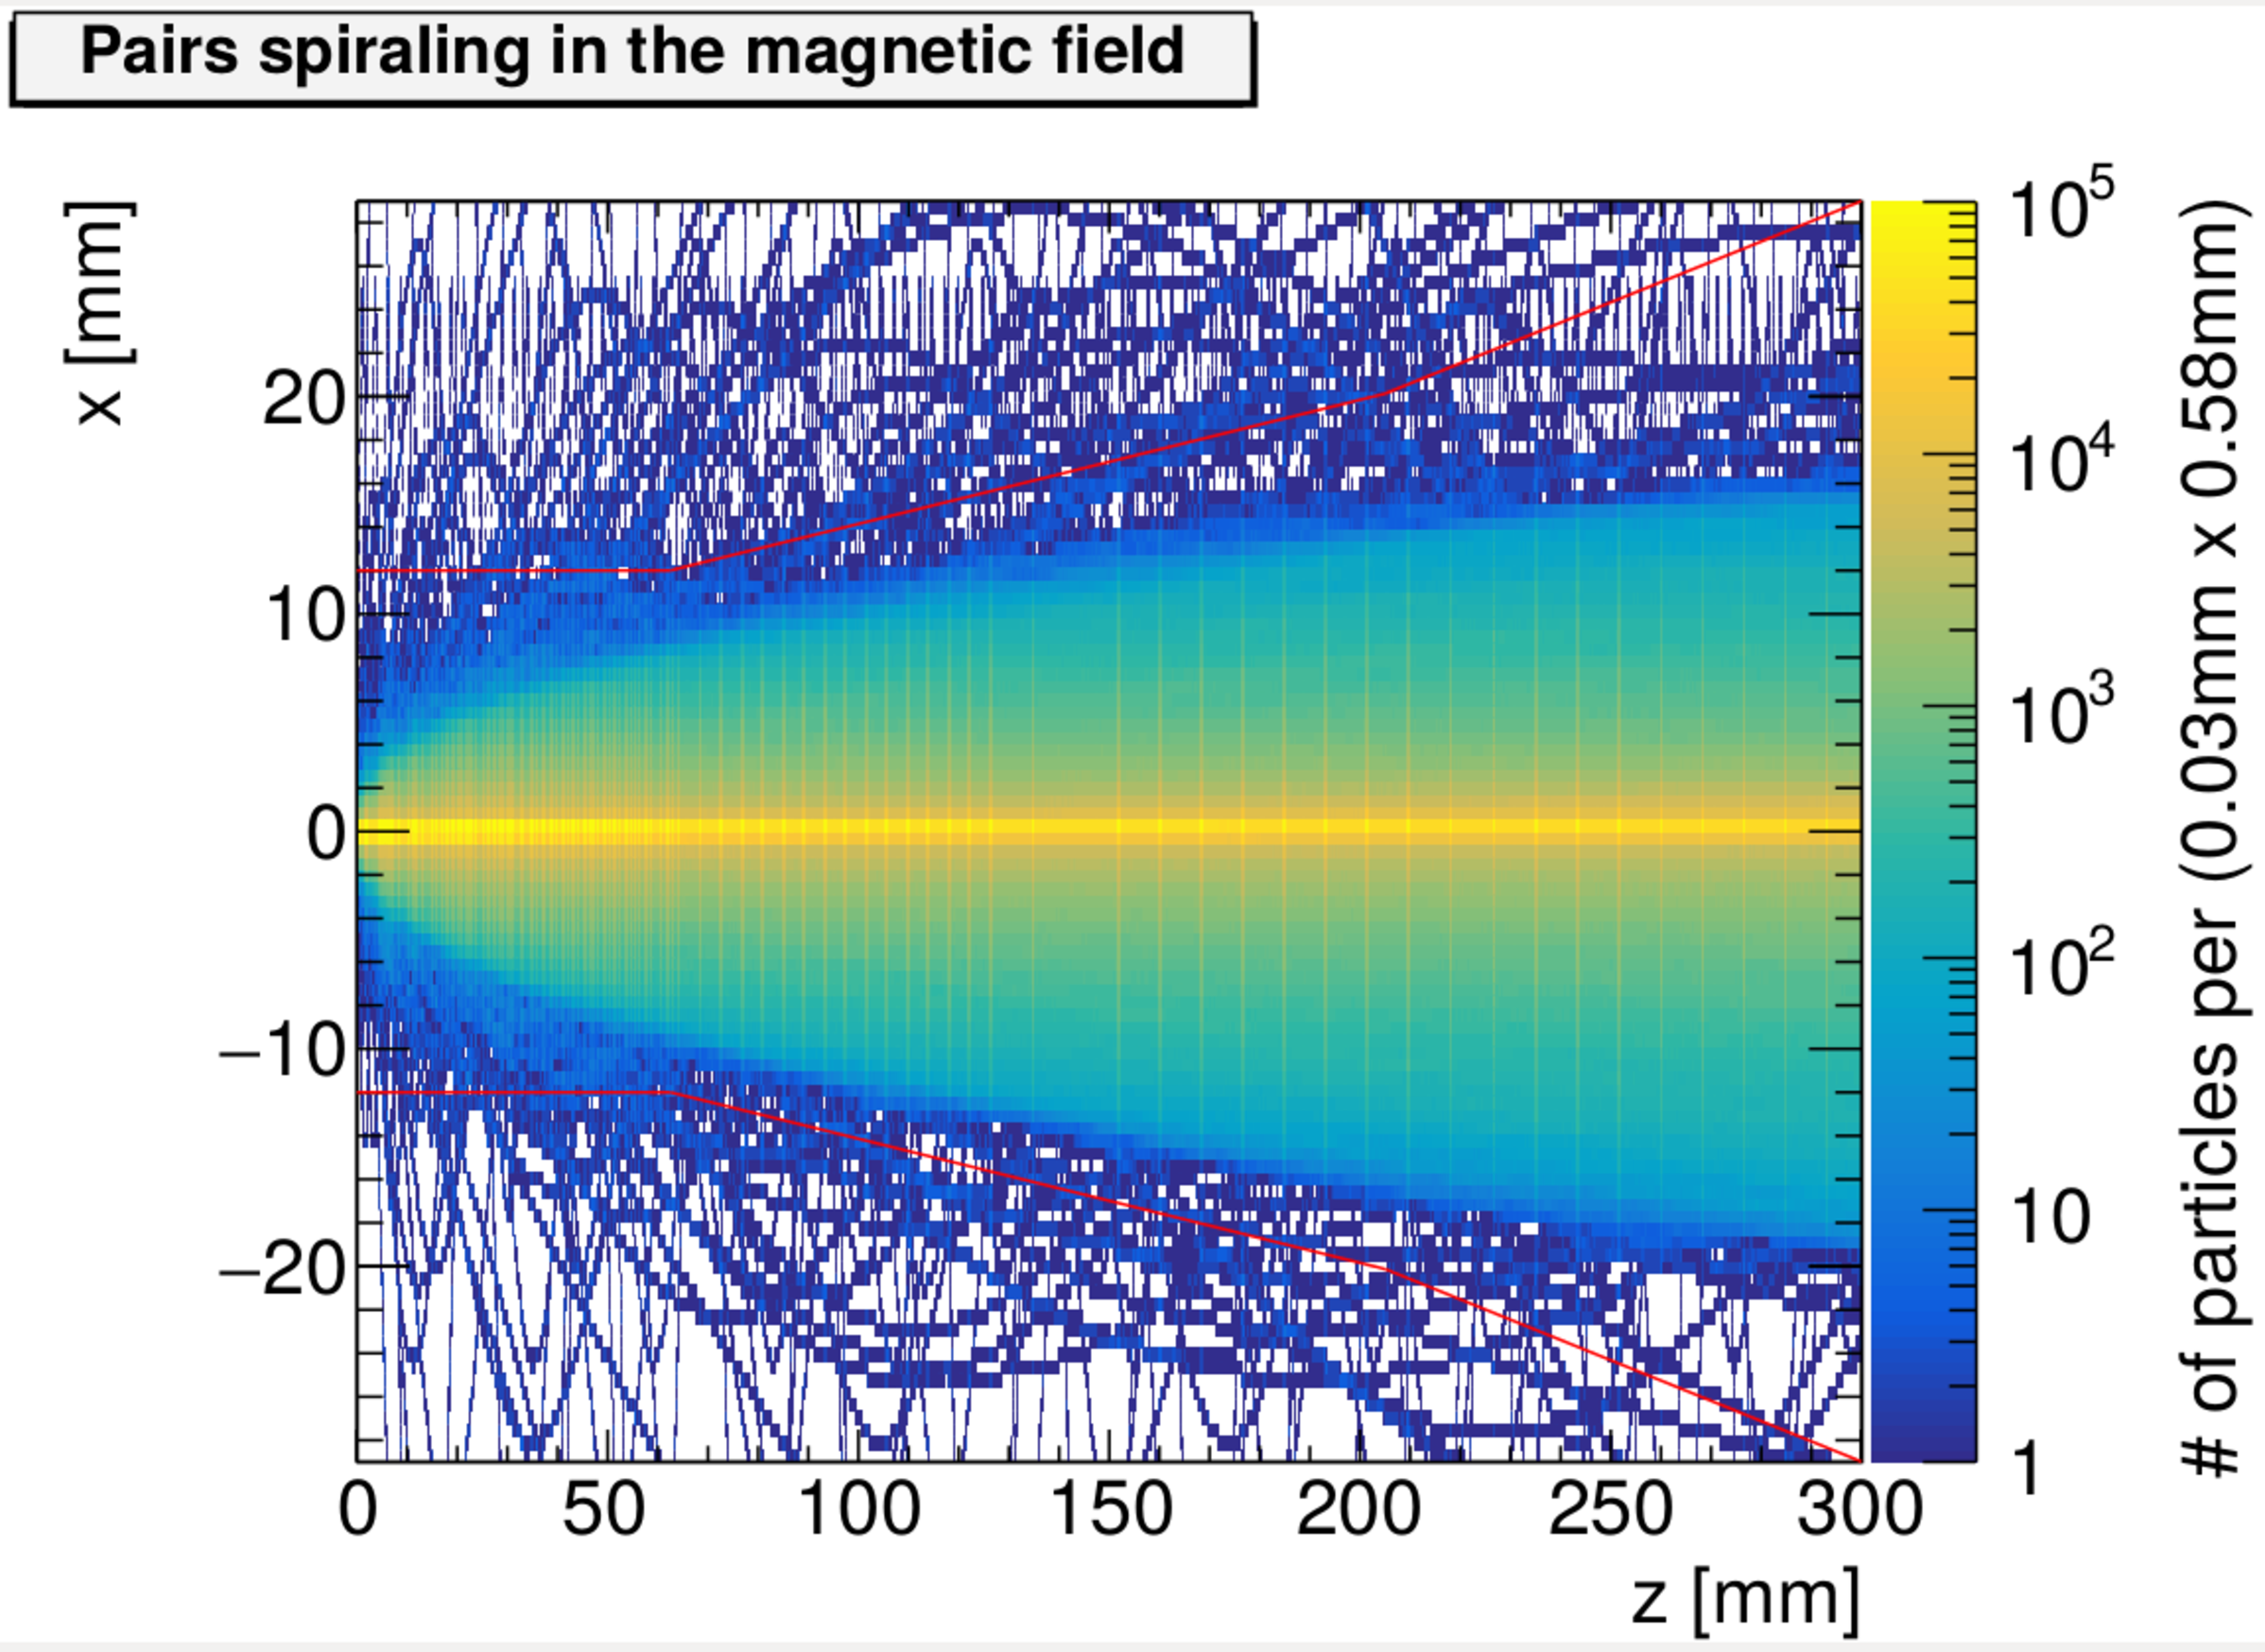
\includegraphics[height=0.26\textheight]{figures/Helix_tracks_xz_1bunch_lowres.pdf}
        \caption{Helix tracks projected on the xz plane}
	\label{fig:helix_xz}
    \end{subfigure}
    \begin{subfigure}[b]{0.49\textwidth}
    \centering
        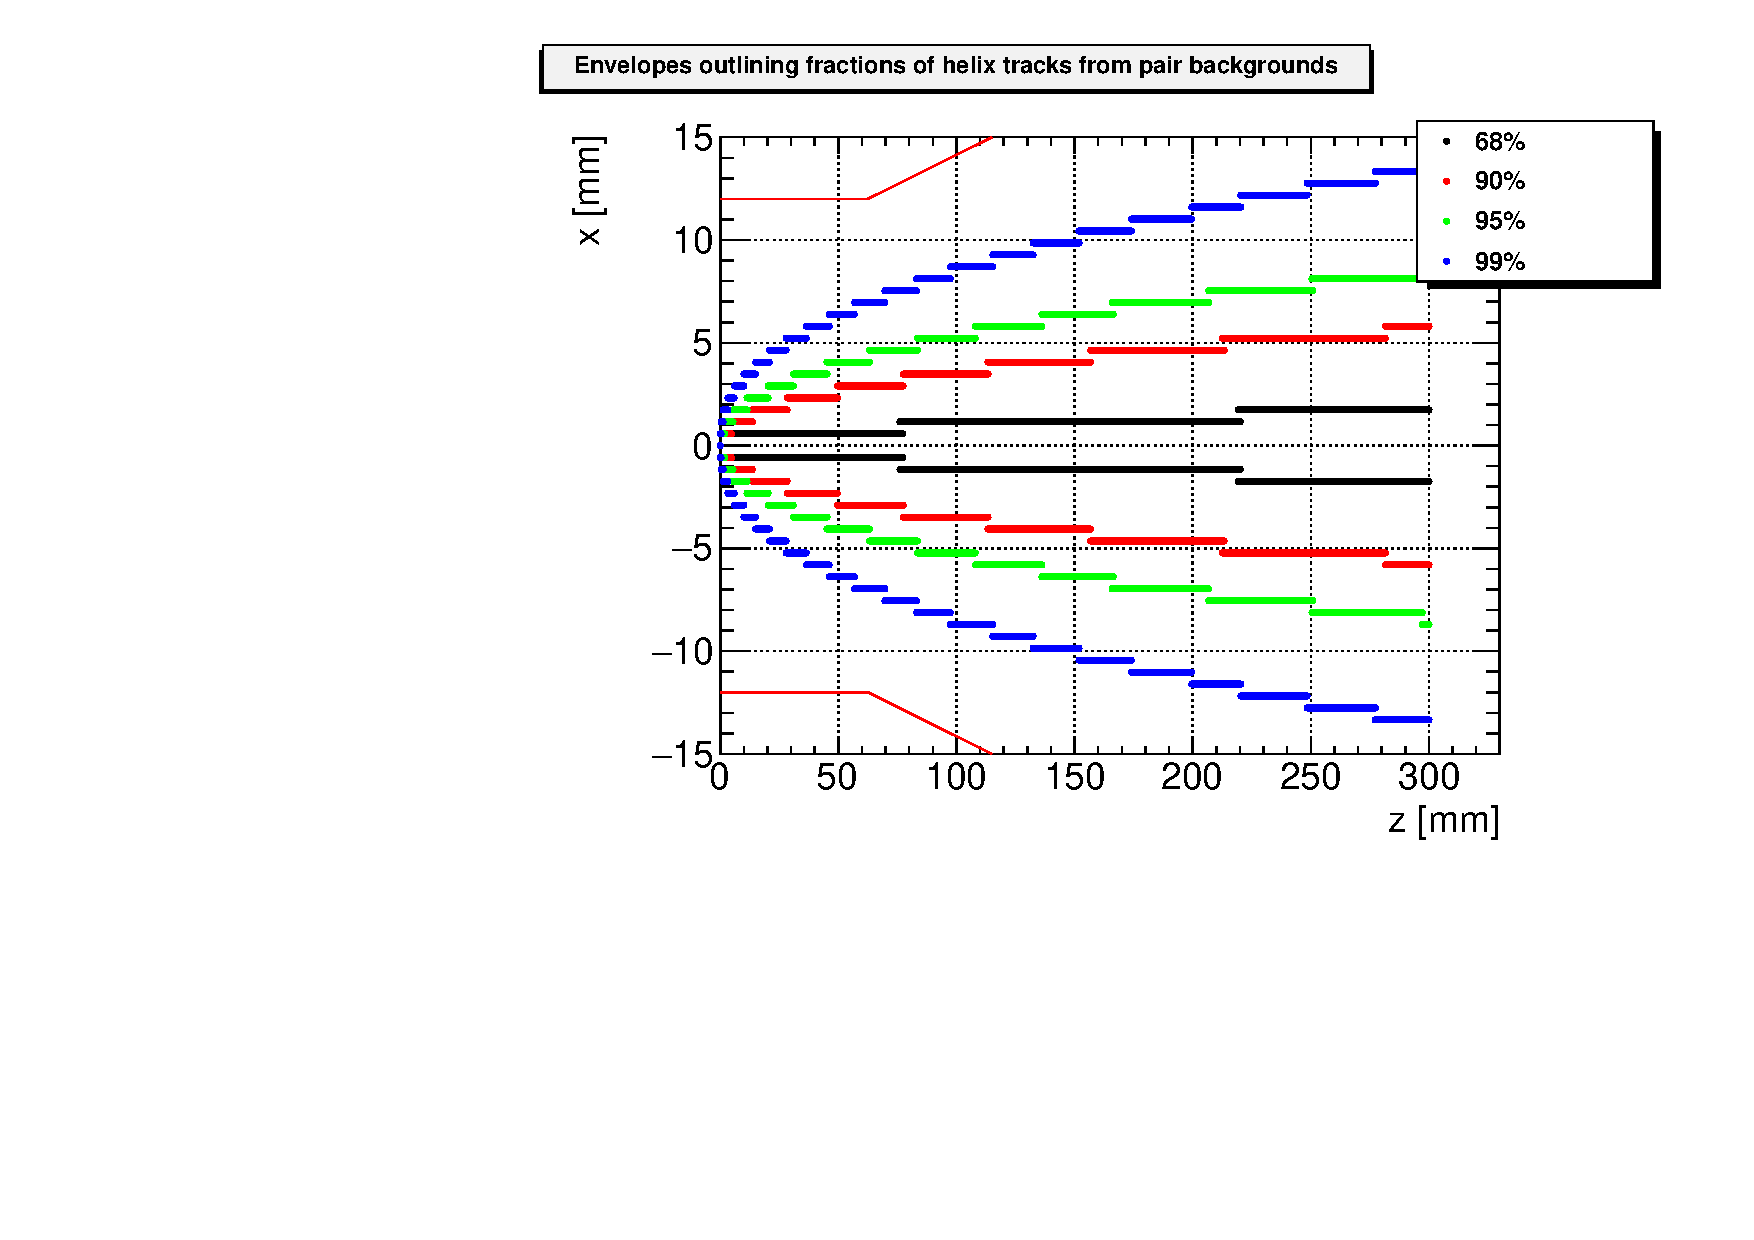
\includegraphics[height=0.26\textheight]{figures/HelixEnvelopes_xz.pdf}
        \caption{Envelopes on the xz plane}
        \label{fig:envelopes_xz}
    \end{subfigure}\\
    \begin{subfigure}[b]{0.49\textwidth}
    \centering
        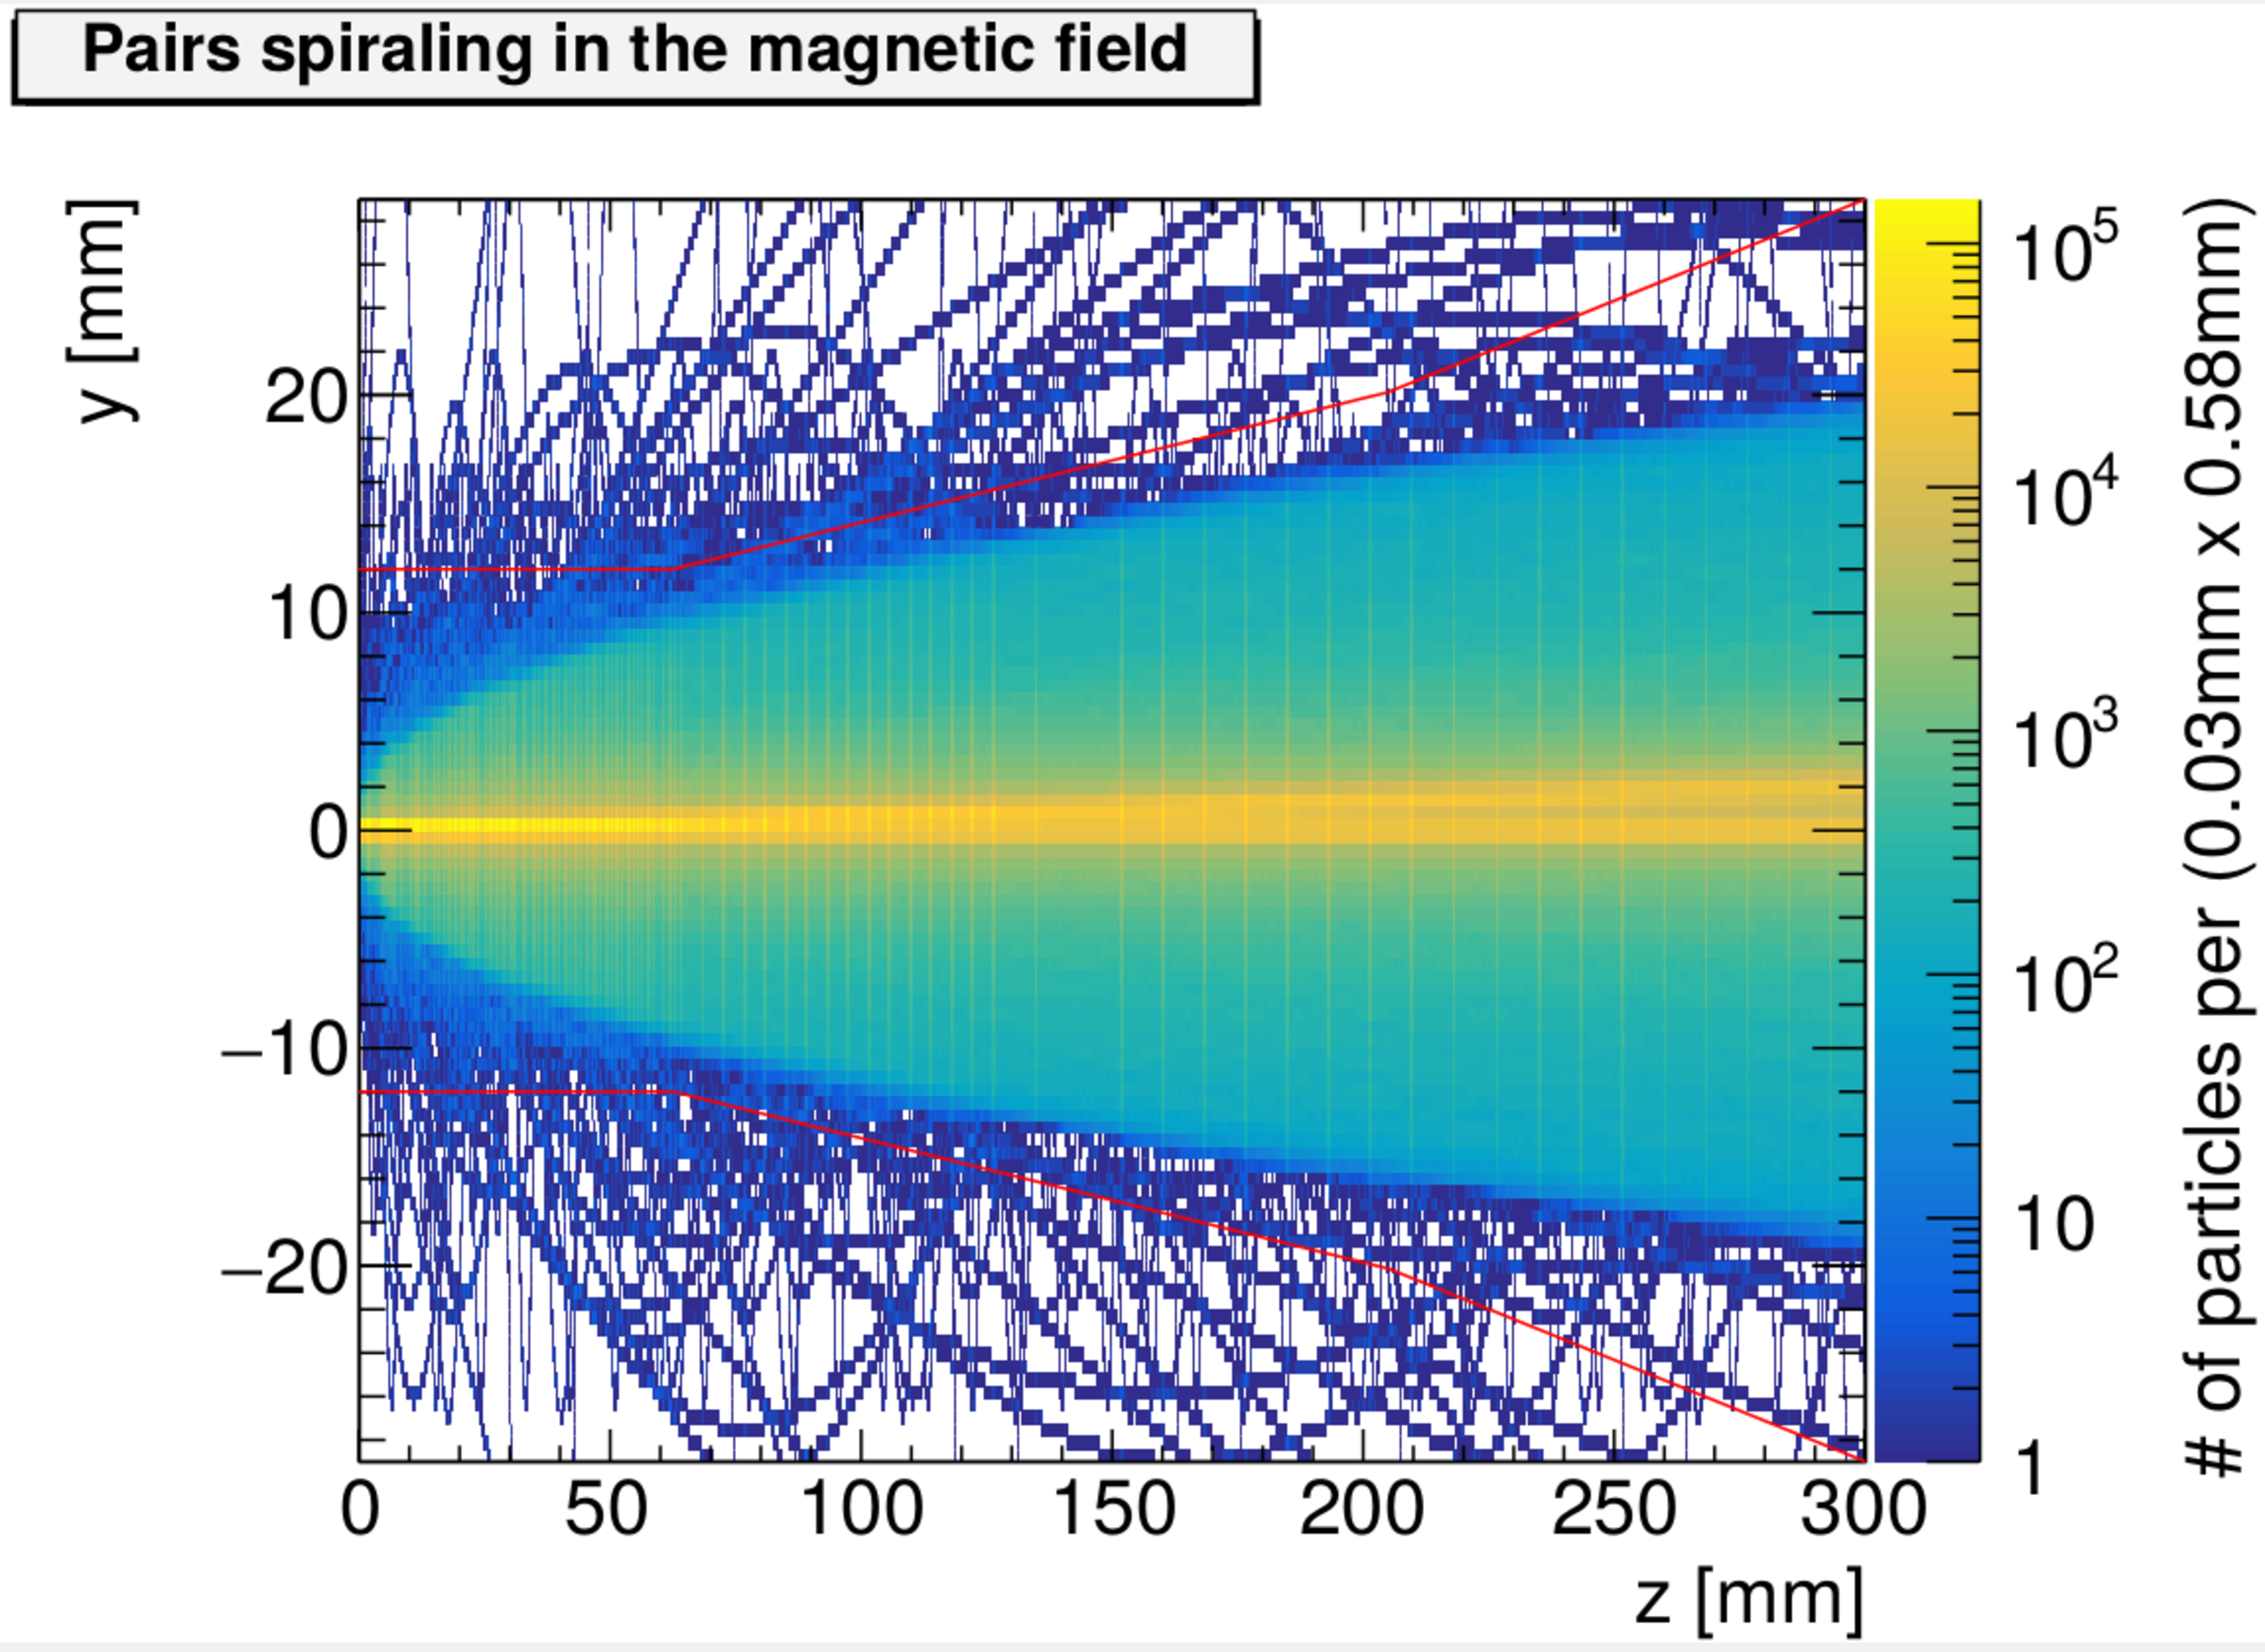
\includegraphics[height=0.26\textheight]{figures/Helix_tracks_yz_1bunch_lowres.pdf}
        \caption{Helix tracks projected on the yz plane}
	\label{fig:helix_yz}
    \end{subfigure}
    \begin{subfigure}[b]{0.49\textwidth}
    \centering
        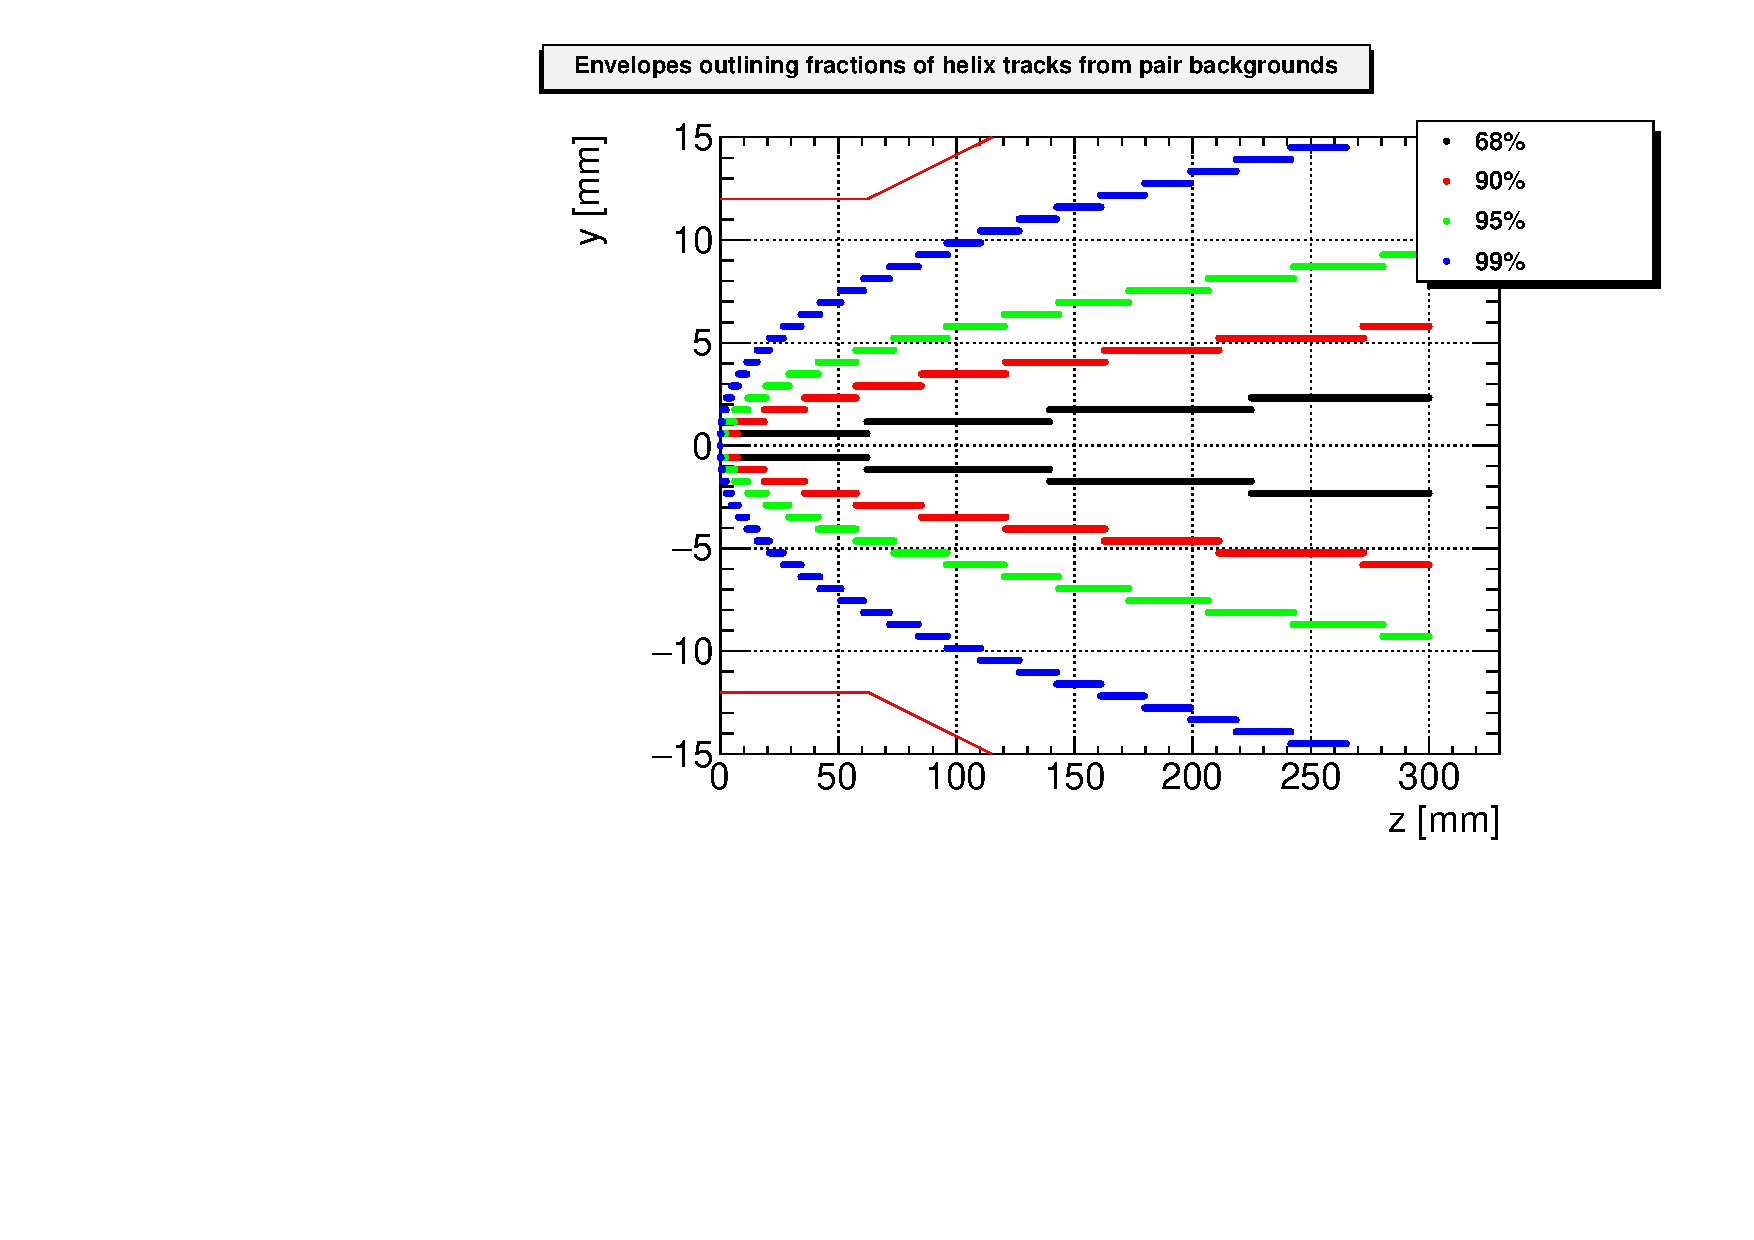
\includegraphics[height=0.26\textheight]{figures/HelixEnvelopes_yz.pdf}
        \caption{Envelopes on the yz plane}
        \label{fig:envelopes_yz}
    \end{subfigure}
    \caption[Helix tracks and their envelopes]{
    The projection of the helix tracks from the pair background particles of one bunch crossing are shown in the xz- and yz-plane in Figures a) and c).
    The color scales shows how many particle tracks are in the single bins of these plots.
    To get a better grasp, Figures b) and d) show the envelopes outlining certain fractions of helix tracks.
    Therefore, the blue line represents the envelope of 99\% of all pair tracks.
    In all subfigures, the thin red lines represent the beam pipe.
    The helix tracks were calculated for a homogeneous magnetic field of \unit{5}\,{T}.
    }
    \label{fig:Helixes}
\end{figure}
\fi